\documentclass{article}

\usepackage{csquotes}
% 使用中文CJK包
\usepackage{CJK}
% 图像插入宏包
\usepackage{graphicx}
% 自定义颜色支持
\usepackage[usenames,dvipsnames]{color}
% 长表格跨页支持
\usepackage{longtable}
% 代码高亮支持
\usepackage{listings}
% 算法伪代码包
\usepackage[ruled,vlined]{algorithm2e}
% 自定义标题格式
\usepackage{titlesec}
% 扩展tabular样式
\usepackage{array}
% 添加页眉页脚
\usepackage{fancyhdr}
% 虚拟正文测试
\usepackage{lipsum}
% 数学环境包
\usepackage{amsmath}
% 首行缩进
\usepackage{indentfirst}
% 树状结构图
\usepackage{tree-dvips}
% 脚注环境
\usepackage{footnote}
% 定制表格线
\usepackage{makecell}
% tikz绘图包
\usepackage{tikz}
% URL超链接
\usepackage[dvips, colorlinks, linkcolor=black]{hyperref}
% 断行URL超链接
\usepackage{breakurl}


% hyperref中文兼容
\pdfstringdefDisableCommands{
\let\CJK@XX\relax
\let\CJK@XXX\relax
\let\CJK@XXXp\relax
\let\CJK@XXXX\relax
\let\CJK@XXXXp\relax
}

\usetikzlibrary{positioning,shapes,shadows,arrows}


% 设置脚注在table中可用
\makesavenoteenv{table}

% 设置标题格式
%\titleformat{\chapter}{\raggedright\Huge\bfseries}{Chapter \thechapter}{1em}{}

% 设置默认字体族, 具体字体请查看texdoc psnfss2e

% 设置Roman字体为Palatino
\renewcommand{\rmdefault}{ppl} 
% 设置TypeWriter字体为Courier
\renewcommand{\ttdefault}{pcr} 

% 设置行距
\setlength{\parskip}{1ex}

% 定义需要的颜色

\definecolor{lightgray}{RGB}{230,230,230}
\definecolor{lightblue}{RGB}{224, 224, 255}
\definecolor{darkblue}{RGB}{192, 192, 255}
\definecolor{lightpink}{RGB}{255, 224, 224}
\definecolor{darkpink}{RGB}{255, 192, 192}
\definecolor{keywordyellow}{RGB}{255, 204, 0}
\definecolor{keywordred}{RGB}{194, 58, 0}
\definecolor{numbercolor}{RGB}{102, 51, 0}

% 设置代码风格

% 定义C语言代码风格
\lstdefinestyle{ccode}
{ 
    language=C, 
    numbers=left, 
    numberstyle=\color{numbercolor},
    basicstyle=\scriptsize\ttfamily\bfseries,
    keywordstyle=\color{blue}, 
    commentstyle=\color{PineGreen},
    stringstyle=\color{red}, 
    frame=shadowbox, 
    frameround=tttt,
    breaklines=true,
    backgroundcolor=\color{lightgray} }

% 定义汇编语言代码风格
\lstdefinestyle{acode}
{ 
    language=,
    morekeywords=[1]{mov, movl, movb, movw, orl, xorw, cli, cld, inb, testb, test, jnz, push, pop, jmp, call, lea, add, sub, ret, jle, outb, ljmp, lgdt},
    morekeywords=[2]{ax, bx, cx, dx, eax, ebx, ecx, edx, cr0, cr1, cr2, cr3, al, ds, es, ss, esp, ebp}, 
    morekeywords=[3]{data, text, bss},
    morekeywords=[4]{long, align, p2align, ascii, fill, globl, space, set, rept, byte, word},
    morecomment=[l]\#,
    numbers=left, 
    numberstyle=\color{numbercolor},
    basicstyle=\scriptsize\ttfamily\bfseries,
    keywordstyle=[1]\color{blue}, 
    keywordstyle=[2]\color{keywordyellow},
    keywordstyle=[3]\color{orange},
    keywordstyle=[4]\color{keywordred},
    commentstyle=\color{PineGreen},
    stringstyle=\color{red}, 
    frame=shadowbox, 
    frameround=tttt,
    breaklines=true,
    backgroundcolor=\color{lightgray} }

    
% 定义命令行输出风格
\lstdefinestyle{console}
{
    language=bash, 
    numbers=none, 
    frame=tRBl,
    basicstyle=\scriptsize\color{green}\ttfamily\bfseries,     
    backgroundcolor=\color{black}}


% 定义exercise输出风格
\lstdefinestyle{exercise}
{
    numbers=none, 
    frame=tRBl,
    breaklines=true,
    breakindent=0pt,
    framexleftmargin=1em,
    framexrightmargin=1em,
    framextopmargin=2ex,
    framexbottommargin=2ex,
    xleftmargin=0.05\linewidth,
    xrightmargin=0.05\linewidth,
    basicstyle=\scriptsize\ttfamily\mdseries,   
    moredelim=[is][\ttfamily\bfseries]{|}{|},
    framerule=0.8pt,
    rulecolor=\color{darkblue}, 
    backgroundcolor=\color{lightblue}}
    

% 定义challenge输出风格
\lstdefinestyle{challenge}
{
    numbers=none, 
    frame=tRBl,
    breaklines=true,
    breakindent=0pt,
    framexleftmargin=1em,
    framexrightmargin=1em,
    framextopmargin=2ex,
    framexbottommargin=2ex,
    xleftmargin=0.05\linewidth,
    xrightmargin=0.05\linewidth,
    basicstyle=\scriptsize\ttfamily\mdseries,   
    moredelim=[is][\ttfamily\bfseries]{|}{|},
    framerule=0.8pt,
    rulecolor=\color{darkpink}, 
    backgroundcolor=\color{lightpink}}
    


% 非常重要, listings关闭非ASCII字符兼容
\lstset{extendedchars=false}


% 定义问题的答案格式
\newcommand{\highlight}[1]{{\bfseries \color{red}  #1}}
% 定义函数名格式
\newcommand{\funcname}[1]{{\ttfamily \small #1}}




\pagestyle{fancy}
\begin{document}
\begin{CJK*}{UTF8}{gkai}

\lhead{操作系统实习报告}
\rhead{张弛, 00848231}
\title{操作系统JOS实习第二次报告}
\author{张弛 \hspace{1ex} 00848231, \\
        zhangchitc@gmail.com}

\maketitle
% 记得在文档末尾插入\clearpage
\tableofcontents
\newpage

\section{Introduction}

我在实验中主要参考了华中科技大学邵志远老师写的JOS实习指导,在邵老师的主页上\burl{http://grid.hust.edu.cn/zyshao/OSEngineering.htm} 可以找到。但是这次实验的指导远远不如lab1的指导详尽,所以我这里需要补充的内容会很多。

\section{Physical Page Management}


\begin{lstlisting}[style=exercise]
|Exercise 1|. In the file kern/pmap.c, you must implement code for the following functions.

        boot_alloc()
	page_init()
	page_alloc()
	page_free()
	
You also need to add some code to i386_vm_init() in pmap.c, as indicated by comments there. For now, just add the code needed leading up to the call to check_page_alloc().

You probably want to work on boot_alloc(), then i386_vm_init(), then page_init(), page_alloc(), and page_free().

check_page_alloc() tests your physical page allocator. You should boot JOS and see whether check_page_alloc() reports success. Fix your code so that it passes. You may find it helpful to add your own assert()s to verify that your assumptions are correct.
\end{lstlisting}

这次实验的内容暂时和页面转换机制没有关系,我们需要重点关注的是物理页面的规划以及管理。主要需要关注JOS内核代码中的inc/queue.h文件以及kern/pmap.c文件。

\subsection{Physical page and its data structure}

请仔细阅读邵老师的讲义中4.3章 第一节 页面管理。其中重点需要掌握以下内容:

\begin{enumerate}
\item{物理页和Page数据结构的对应关系}
\item{对Page*页面链表的宏操作,在inc/queue.h中}
\end{enumerate}

里面我唯一碰到的问题就是没看懂为什么JOS给出的链表模板要写成下面这样的形式:

\begin{lstlisting}[style=ccode, firstnumber=165, title={\scriptsize \ttfamily \bfseries inc/queue.h}]
/*
 * Reset the list named "head" to the empty list.
 */
#define	LIST_INIT(head) do {						\
	LIST_FIRST((head)) = NULL;					\
} while (0)
\end{lstlisting}

这个宏的的目的是将链表初始化为空。但我奇怪的是为什么要写成一个只执行一次的while循环的形式,而不是直接大括号包住这一段语句就可以了? 实验室的白光东师兄给出了一个详尽满意的答案。他给了我下面这样的程序:

\begin{lstlisting}[style=ccode, title={\scriptsize \ttfamily \bfseries test.c}]
#include <stdio.h>

#define MACRO() do { \
  printf ("hello\n"); \
} while (0)

int main () {
  int x;
  scanf ("%d\n", &x);

  if (x) 
    MACRO ();
  else
    printf ("this is else\n");
  return 0;
}
\end{lstlisting}

然后使用gcc -E test.c编译这段程序,参数E的目的是为了让编译器仅仅进行预编译以后即停下来,并输出预编译后的程序结果,那么我们得到这样的输出

\begin{lstlisting}[style=console]
int main () {
  int x;
  scanf ("%d\n", &x);

  if (x)
    do { printf ("hello\n"); } while (0);
  else
    printf ("this is else\n");
  return 0;
}
zhangchi@zhangchi-desktop:/tmp/test$ 
\end{lstlisting}

很明显我们看到相关的\funcname{MACRO ();}调用变成了其相应的宏展开,请特别注意,调用的时候我们是以单个语句的形式调用\funcname{MACRO ()}的,那么展开以后的形式还是满足了单个语句(一个while循环),并且,在其后面加上了分号。如果我们把MACRO改成:

\begin{lstlisting}[style=ccode, title={\scriptsize \ttfamily \bfseries test.c}]
#define MACRO() { \
  printf ("hello\n"); \
}
\end{lstlisting}

那么再次展开的结果会变成:


\begin{lstlisting}[style=console]
int main () {
  int x;
  scanf ("%d\n", &x);

  if (x)
    { printf ("hello\n"); };
  else
    printf ("this is else\n");
  return 0;
}
zhangchi@zhangchi-desktop:/tmp/test$ 
\end{lstlisting}

明显可以看出这样的转换造成语法错误,用大括号包裹的代码块后不需要分号。这里出错的原因就在于我们调用\funcname{MACRO ()}之前是当成一个单个语句,调用展开后变成了一个代码块。那么相应的语法结构就出现了变化导致出错。

真是考虑得非常细致!感谢师兄!

\subsection{Physical memory layout}

请仔细阅读邵老师的讲义中的4.3章 第一节 页面管理 中``页面管理链表在内存中的存储和放置''小节。重点理解

\begin{enumerate}
\item{pages数组和Page*链表的对应关系}
\item{pages所在的空间是怎样分配的}
\item{整个物理内存的布局}
\end{enumerate}

这里要说的是,在做完lab1以后,我们知道了在实模式下物理页面前640KB的一些分配情况,如BIOS的载入地址、boot loader载入地址、操作系统内核ELF文件头的临时存放空间等等,具体的布局应该如下图所示:

\begin{figure}[htp]
\centering
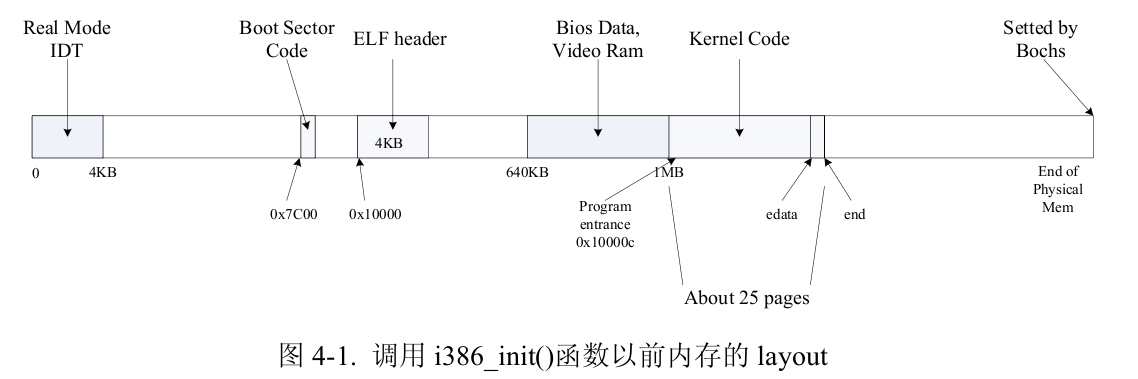
\includegraphics[scale=0.320]{/home/zhangchi/lab/report/screen1.png}
\end{figure}

在lab1完成后,我们从0x000100000这个位置放入内核,直到end结束。end是链接器作链接时得到的内核结束地址。

那么在建立物理页面对应的Page* 链表时,我们需要为这个链表分配实际的物理内存空间,在二级页地址映射机制中,系统还需要一个页目录存下所有二级页表的地址,这个也是需要操作系统预先分配空间的,所以结合上图,我们第一步完成之后物理内存布局应该如下图所示:


\begin{figure}[htp]
\centering
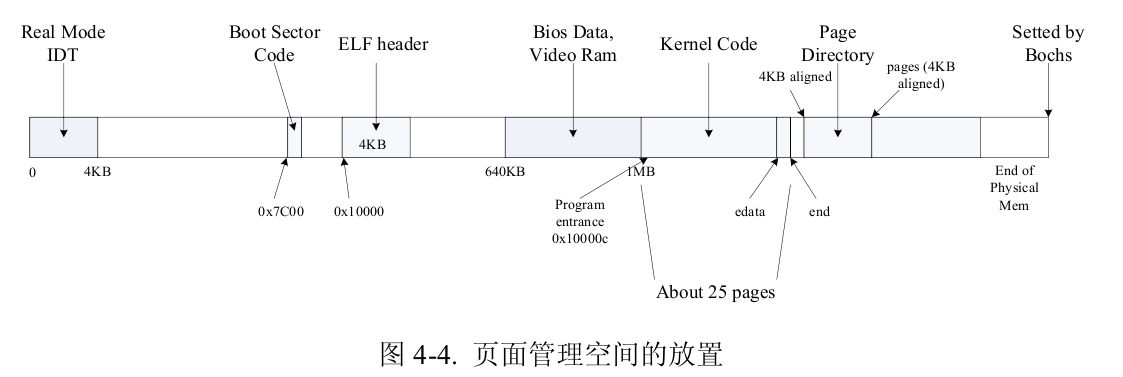
\includegraphics[scale=0.320]{/home/zhangchi/lab/report/screen2.png}
\label{physmemlayout}
\end{figure}

我们第一步的目的就是为页目录和pages分配好空间,并建立起空闲页表page\_free\_list。


开始写代码的时候,首先需要弄清楚kern/pmap.c中的几个基本的变量:

\begin{lstlisting}[style=ccode, firstnumber=12, title={\scriptsize \ttfamily \bfseries kern/pmap.c}]
// These variables are set by i386_detect_memory()
static physaddr_t maxpa;	// Maximum physical address
size_t npage;			// Amount of physical memory (in pages)
static size_t basemem;		// Amount of base memory (in bytes)
static size_t extmem;		// Amount of extended memory (in bytes)

// These variables are set in i386_vm_init()
pde_t* boot_pgdir;		// Virtual address of boot time page directory
physaddr_t boot_cr3;		// Physical address of boot time page directory
static char* boot_freemem;	// Pointer to next byte of free mem

struct Page* pages;		// Virtual address of physical page array
static struct Page_list page_free_list;	// Free list of physical pages
\end{lstlisting}

这里只需要知道两个变量,boot\_freemem和boot\_pgdir,前者是当前可用内存的开始地址(也就是说,内核载入以后,系统管理所需要的内容就从end以后开始分配,即从一开始boot\_freemem是等于end,这个在接下来的代码里就能看到);boot\_pgdir则是系统页目录所在空间的开始地址。\highlight{注意,两者地址都是虚拟地址!在这次lab中一定要搞清楚的一个细节就是虚拟地址,线性地址和物理地址的区别,以及我们使用的地址变量哪些是虚拟地址,哪些是物理地址。}


接下来我们可以看到\funcname{i386\_vm\_init ()},从这里开始我们这次的lab。一开始就看到关于页目录的初始化代码:

\begin{lstlisting}[style=ccode, title={\scriptsize \ttfamily \bfseries kern/pmap.c: i386\_vm\_init ()}]
	//////////////////////////////////////////////////////////////////////
	// create initial page directory.
	pgdir = boot_alloc(PGSIZE, PGSIZE);

	memset(pgdir, 0, PGSIZE);
	boot_pgdir = pgdir;
	boot_cr3 = PADDR(pgdir);
\end{lstlisting}

其中\funcname{boot\_alloc ()}为其分配内存空间地址,然后将分配的地址段清空。然后将其物理地址(PADDR)放入boot\_cr3准备启动x86的页面地址转换机制。这里要注意几点:

\begin{itemize}
\item{从\funcname{boot\_alloc ()}得到的页面是不会作相应的初始化工作的,所以如果对分配到的空间有要求清空,必须自己亲自动手}
\item{\funcname{memset}接受的清空地址是pgdir即一个虚拟地址,这个在我们后面的工作中对实际分配到的\highlight{物理页面}进行初始化时提醒,清空时使用\funcname{memset}也一定要使用实际物理页面对应的\highlight{内核虚拟地址}}
\item{boot\_cr3得到的是一个\highlight{物理地址},这个和我们前面强调的分清每个地址变量到底是虚拟地址还是物理地址有密切联系}
\end{itemize}

接下来我们来看一下第一个需要实现的函数\funcname{boot\_alloc ()}

\begin{lstlisting}[style=ccode, title={\scriptsize \ttfamily \bfseries kern/pmap.c: boot\_alloc ()}]
static void*
boot_alloc(uint32_t n, uint32_t align)
{
	extern char end[];
	void *v;

	// Initialize boot_freemem if this is the first time.
	// 'end' is a magic symbol automatically generated by the linker,
	// which points to the end of the kernel's bss segment -
	// i.e., the first virtual address that the linker
	// did _not_ assign to any kernel code or global variables.
	if (boot_freemem == 0)
		boot_freemem = end;

	// LAB 2: Your code here:
	//	Step 1: round boot_freemem up to be aligned properly
	//		(hint: look in types.h for some handy macros)
	//	Step 2: save current value of boot_freemem as allocated chunk
	//	Step 3: increase boot_freemem to record allocation
	//	Step 4: return allocated chunk

    	v = ROUNDUP (boot_freemem, align);
    	boot_freemem = (char*) v + n;
    
	return v;
}
\end{lstlisting}

这个函数的问题不大。

看接下来的代码:

\begin{lstlisting}[style=ccode, title={\scriptsize \ttfamily \bfseries kern/pmap.c: i386\_vm\_init ()}]
	//////////////////////////////////////////////////////////////////////
	// Recursively insert PD in itself as a page table, to form
	// a virtual page table at virtual address VPT.
	// (For now, you don't have understand the greater purpose of the
	// following two lines.)

	// Permissions: kernel RW, user NONE
	pgdir[PDX(VPT)] = PADDR(pgdir)|PTE_W|PTE_P;

	// same for UVPT
	// Permissions: kernel R, user R 
	pgdir[PDX(UVPT)] = PADDR(pgdir)|PTE_U|PTE_P;

	//////////////////////////////////////////////////////////////////////
	// Allocate an array of npage 'struct Page's and store it in 'pages'.
	// The kernel uses this array to keep track of physical pages: for
	// each physical page, there is a corresponding struct Page in this
	// array.  'npage' is the number of physical pages in memory.
	// User-level programs will get read-only access to the array as well.
	// Your code goes here:
	

	pages = boot_alloc (npage * sizeof (struct Page), PGSIZE);

	//////////////////////////////////////////////////////////////////////
	// Now that we've allocated the initial kernel data structures, we set
	// up the list of free physical pages. Once we've done so, all further
	// memory management will go through the page_* functions. In
	// particular, we can now map memory using boot_map_segment or page_insert
	page_init();

	check_page_alloc();

	page_check();
\end{lstlisting}

前两句对pgdir的操作我们可以先不用管他,在后来设置页表的时候我们会回过头来看这两句话的含义。在23行里为pages分配空间以后,就进入倒\funcname{page\_init ()}对链表进行初始化了。

在进行接下来的编码之前,我们先需要了解JOS对于地址编码的一些规定,在inc/mmu.h中,我们可以找到一组详尽的宏:

\begin{lstlisting}[style=ccode, firstnumber=16, title={\scriptsize \ttfamily \bfseries inc/mmu.h}]
// A linear address 'la' has a three-part structure as follows:
//
// +--------10------+-------10-------+---------12----------+
// | Page Directory |   Page Table   | Offset within Page  |
// |      Index     |      Index     |                     |
// +----------------+----------------+---------------------+
//  \--- PDX(la) --/ \--- PTX(la) --/ \---- PGOFF(la) ----/
//  \----------- PPN(la) -----------/
//
// The PDX, PTX, PGOFF, and PPN macros decompose linear addresses as shown.
// To construct a linear address la from PDX(la), PTX(la), and PGOFF(la),
// use PGADDR(PDX(la), PTX(la), PGOFF(la)).

// page number field of address
#define PPN(la)		(((uintptr_t) (la)) >> PTXSHIFT)
#define VPN(la)		PPN(la)		// used to index into vpt[]

// page directory index
#define PDX(la)		((((uintptr_t) (la)) >> PDXSHIFT) & 0x3FF)
#define VPD(la)		PDX(la)		// used to index into vpd[]

// page table index
#define PTX(la)		((((uintptr_t) (la)) >> PTXSHIFT) & 0x3FF)

// offset in page
#define PGOFF(la)	(((uintptr_t) (la)) & 0xFFF)

// construct linear address from indexes and offset
#define PGADDR(d, t, o)	((void*) ((d) << PDXSHIFT | (t) << PTXSHIFT | (o)))
\end{lstlisting}


其中PDX,PTX和PGOFF都很好理解,需要注意的是PPN,一个\highlight{线性地址}的PPN其实没有什么意义,但是如果我们对一个\highlight{物理地址}取PPN的话,就可以利用这个PPN直接访问\highlight{这个物理地址在pages数组中的对应页}!这个宏所以非常的好用。

我们来看到前面提到对物理页面链表进行初始化的\funcname{page\_init ()} 过程:



\begin{lstlisting}[style=ccode, title={\scriptsize \ttfamily \bfseries kern/pmap.c: boot\_init ()}]
//
// Initialize page structure and memory free list.
// After this is done, NEVER use boot_alloc again.  ONLY use the page
// allocator functions below to allocate and deallocate physical
// memory via the page_free_list.
//
void
page_init(void)
{
    // The example code here marks all physical pages as free.
    // However this is not truly the case.  What memory is free?
    //  1) Mark physical page 0 as in use.
    //     This way we preserve the real-mode IDT and BIOS structures
    //     in case we ever need them.  (Currently we don't, but...)
    //  2) The rest of base memory, [PGSIZE, basemem) is free.
    //  3) Then comes the IO hole [IOPHYSMEM, EXTPHYSMEM).
    //     Mark it as in use so that it can never be allocated.
    //  4) Then extended memory [EXTPHYSMEM, ...).
    //     Some of it is in use, some is free. Where is the kernel
    //     in physical memory?  Which pages are already in use for
    //     page tables and other data structures?
    //
    // Change the code to reflect this.
    //

    int i;
    int lower_ppn = PPN (IOPHYSMEM);
    int upper_ppn = PPN (ROUNDUP (boot_freemem, PGSIZE));

    LIST_INIT(&page_free_list);
    for (i = 0; i < npage; i++) {
        pages[i].pp_ref = 0;

        if (i == 0) continue;
        if (lower_ppn <= i && i < upper_ppn) continue;
 
        LIST_INSERT_HEAD(&page_free_list, &pages[i], pp_link);
    }
}
\end{lstlisting}

这个函数的具体工作就是建立其每个物理页面对应的实际链表节点,然后把那些被操作系统占用或是系统预留空间从链表里去除掉。通过对照\ref{physmemlayout}中提到的物理内存的使用布局,可以总结出以下几个使用的物理地址区域:


\begin{description}
\item[$[0, \mathrm{PGSIZE})$] :\newline
中断向量表IDT以及BIOS的相关载入程序
\item[$[0, \text{PGSIZE})$] \
中断向量表IDT以及BIOS的相关载入程序

\end{description}

\begin{align}
[0, \text{PGSIZE}) &: \text{中断向量表IDT以及BIOS的相关载入程序} \notag \\
[\mathrm{IOPHYSMEM}, \mathrm{EXTPHYSMEM}) &: 用来 \notag
\end{align}


\begin{lstlisting}[style=ccode, title={\scriptsize \ttfamily \bfseries kern/pmap.c: boot\_alloc ()}]
\end{lstlisting}

\begin{lstlisting}[style=ccode, title={\scriptsize \ttfamily \bfseries kern/pmap.c: boot\_alloc ()}]
\end{lstlisting}

\begin{lstlisting}[style=ccode, title={\scriptsize \ttfamily \bfseries kern/pmap.c: boot\_alloc ()}]
\end{lstlisting}

\begin{lstlisting}[style=ccode, title={\scriptsize \ttfamily \bfseries kern/pmap.c: boot\_alloc ()}]
\end{lstlisting}

\begin{lstlisting}[style=ccode, title={\scriptsize \ttfamily \bfseries kern/pmap.c: boot\_alloc ()}]
\end{lstlisting}

\begin{lstlisting}[style=ccode, title={\scriptsize \ttfamily \bfseries kern/pmap.c: boot\_alloc ()}]
\end{lstlisting}

\begin{lstlisting}[style=ccode, title={\scriptsize \ttfamily \bfseries kern/pmap.c: boot\_alloc ()}]
\end{lstlisting}




\begin{lstlisting}[style=console]
\end{lstlisting}

\begin{lstlisting}[style=console]
\end{lstlisting}

\begin{lstlisting}[style=console]
\end{lstlisting}

\begin{lstlisting}[style=console]
\end{lstlisting}

\begin{lstlisting}[style=console]
\end{lstlisting}



\begin{lstlisting}[style=exercise]
\end{lstlisting}

\begin{lstlisting}[style=exercise]
\end{lstlisting}

\begin{lstlisting}[style=exercise]
\end{lstlisting}

\begin{lstlisting}[style=exercise]
\end{lstlisting}

\begin{lstlisting}[style=exercise]
\end{lstlisting}

\begin{lstlisting}[style=exercise]
\end{lstlisting}


\begin{lstlisting}[style=challenge]
\end{lstlisting}

\begin{lstlisting}[style=challenge]
\end{lstlisting}

\begin{lstlisting}[style=challenge]
\end{lstlisting}





\begin{lstlisting}[style=acode, firstnumber=44, title={\scriptsize \ttfamily \bfseries boot/boot.S}]
\end{lstlisting}

\begin{lstlisting}[style=acode, firstnumber=44, title={\scriptsize \ttfamily \bfseries boot/boot.S}]
\end{lstlisting}

\begin{lstlisting}[style=acode, firstnumber=44, title={\scriptsize \ttfamily \bfseries boot/boot.S}]
\end{lstlisting}

\begin{lstlisting}[style=acode, firstnumber=44, title={\scriptsize \ttfamily \bfseries boot/boot.S}]
\end{lstlisting}

\begin{lstlisting}[style=acode, firstnumber=44, title={\scriptsize \ttfamily \bfseries boot/boot.S}]
\end{lstlisting}


\begin{lstlisting}[style=ccode, firstnumber=44, title={\scriptsize \ttfamily \bfseries boot/boot.S}]
\end{lstlisting}




\clearpage

\end{CJK*}
\end{document}
	

